\documentclass{article}
\usepackage[utf8]{inputenc}
\RequirePackage[left=1.5cm,top=1cm,right=1.5cm,bottom=2cm,nohead,nofoot]{geometry}
\title{Assignment-5}
\author{Urbi Ghosh}
\date{March 2021}

\usepackage{natbib}
\usepackage{graphicx}

\begin{document}

\maketitle

\section{Introduction}
Sir Lewis Hamilton is a British Formula One racing driver. He has won record-equalling seven world championships to date, with more wins than any other driver in the history of Formula One. His story is even more interesting as he is the only black driver to race in the sport.  With an impressive fourteen-year career (and counting), there is a plethora of data on his performances in different tracks, under different constructors, different weather conditions, etc, and even comparisons with other legendary drivers like Michael Schumacher.
\begin{figure}[h]
\centering
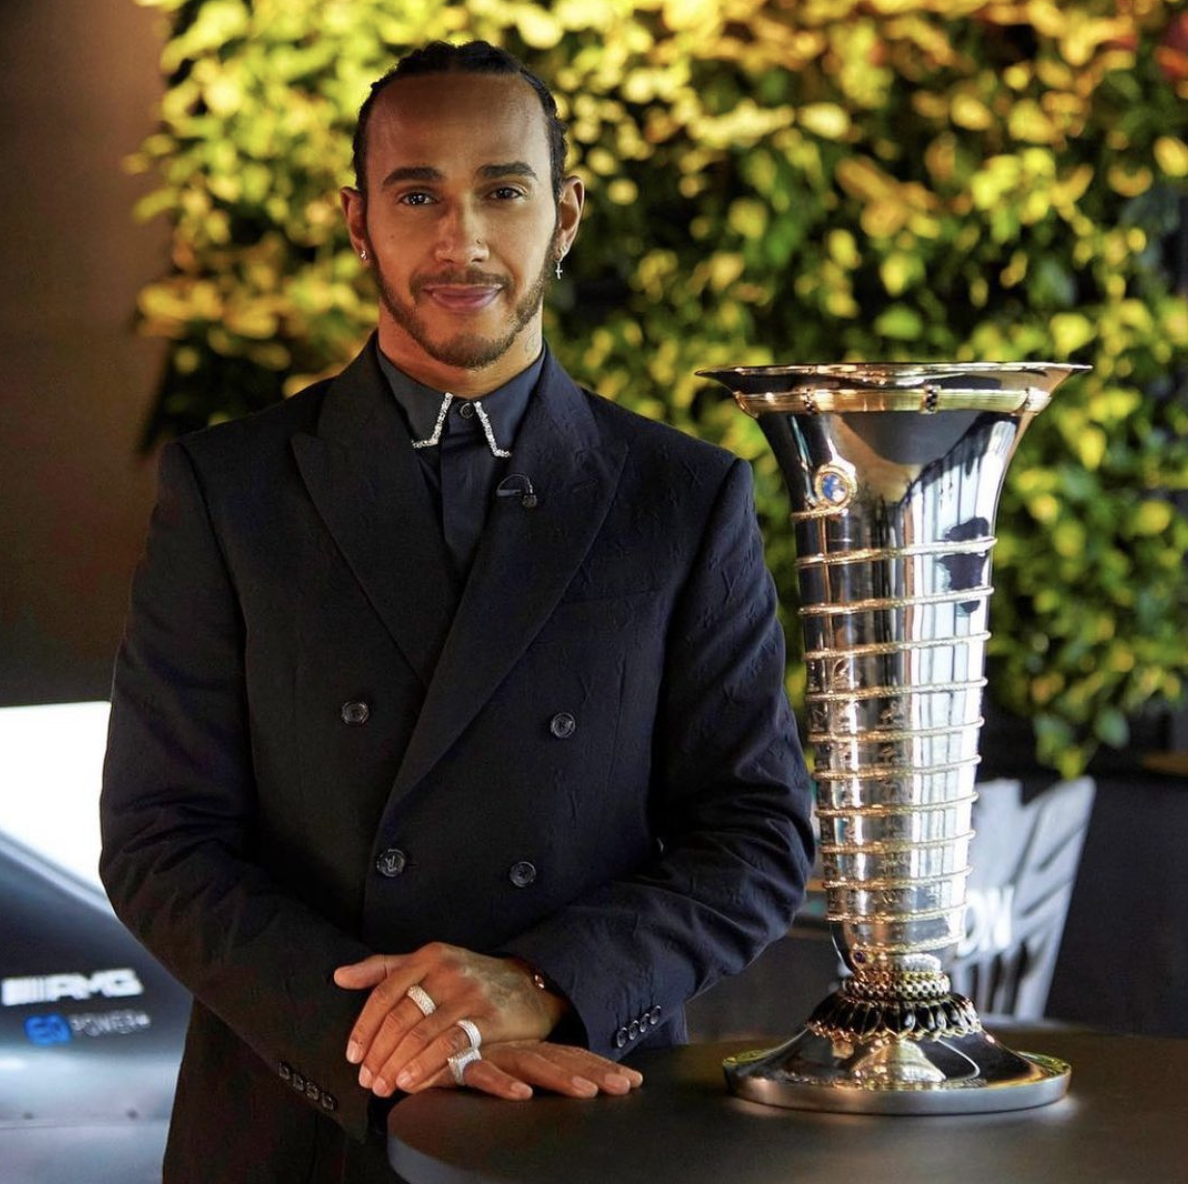
\includegraphics[scale=0.3]{lh}
\caption{Hamilton receiving the BBC Sportsman of the year award 2020}
\label{fig:lh}
\end{figure}
\\
\section{Season-wise and overall Performance Analysis}
The following bar graph represents the data for his ranks in seasons starting from his debut (2007) to present (2020).\\
\begin{figure}[h!]
\centering
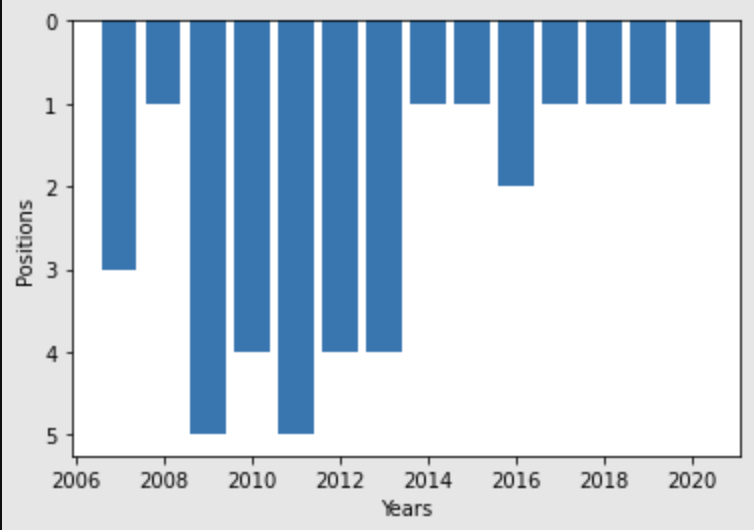
\includegraphics[scale=0.5]{bar}
\caption{}
\label{fig:bar}
\end{figure}\\\\\\\\\\\\\
The exploded pie chart shows a comparison of the finishing positions he has secured over all his races till date. A grid in Formula one consists of twenty racers, hence allows ranks from 1 to 20. Generally low ranks by experienced drivers like Hamilton are caused because of mid race crashes or  spin offs.
\begin{figure}[h!]
\centering
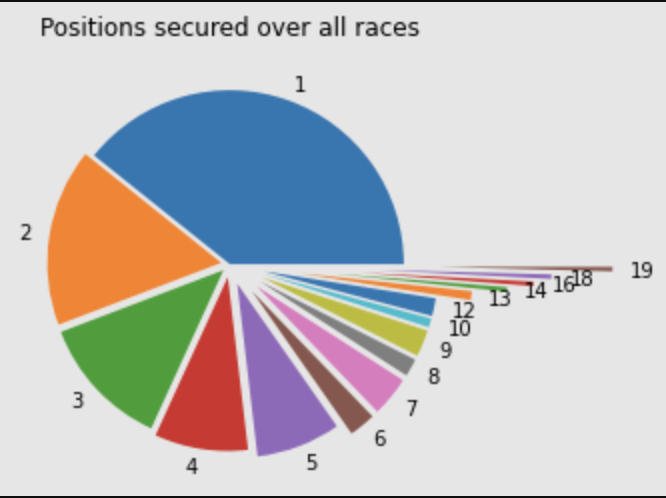
\includegraphics[scale=0.6]{pie}
\caption{}
\label{fig:pie}
\end{figure}
\section{Analysis of track-wise performance}
Tracks have a major impact on drivers. Some tracks have long straights, some have lots of successive turns. Some tracks are prone to rains, dust-storms etc and some are too narrow to allow overtaking. The analysis can be done best with a heat map so that track-wise and year-wise performance trends can be observed simultaneously and distinctly.
\begin{figure}[h!]
\centering
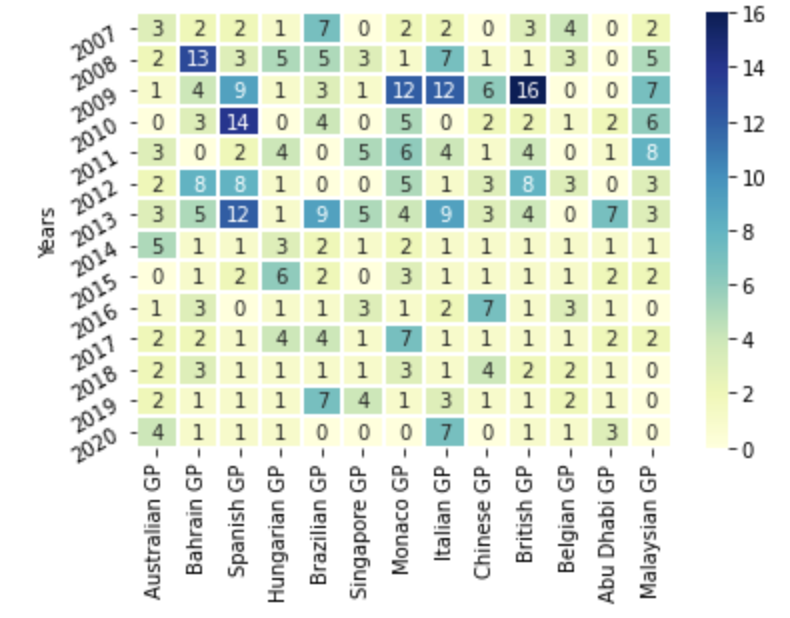
\includegraphics[scale=0.75]{track}
\caption{}
\label{fig:track}
\end{figure}\\\\\\
\section{Transition from McLaren to Mercedes}
The most controversial career decision taken by Hamilton, was his transition from the then leading team McLaren to the then-mediocre team Mercedes, in 2013. 2014 saw the rise of the turbo hybrid era and the rise of Mercedes which provided the perfect platform for Hamilton to secure his four consecutive world championship wins.
%scatter plot, position vs race
\begin{figure}[h!]
\centering
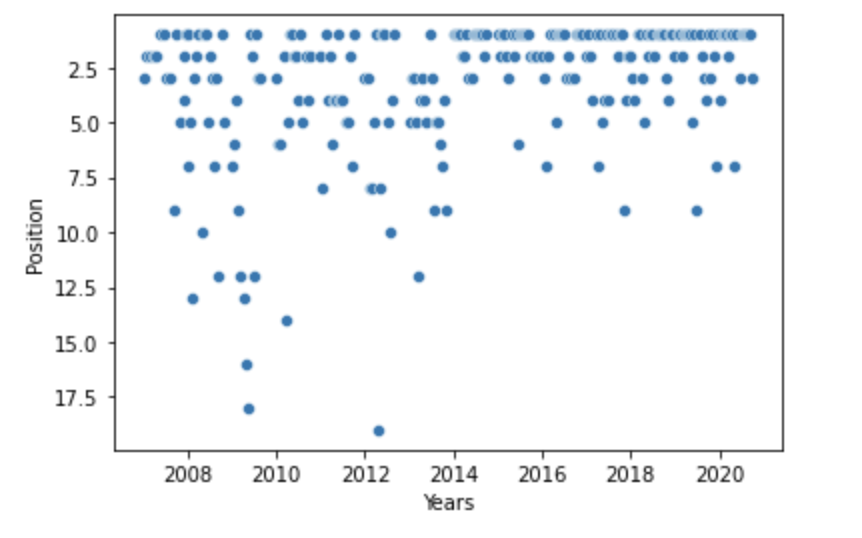
\includegraphics[scale=0.8]{scatter}
\caption{}
\label{fig:scatter}
\end{figure}
\section{A comparison with Schumacher}
An analysis of Hamilton's on track career is incomplete without the comparison between the greatest drivers of their generation. Before the coming of Hamilton, it was widely believed that Schumacher was the greatest drivers of all times, with his then unbeaten record of seven world championship wins, and 92 race wins. 
\\
\begin{figure}[h]
\centering
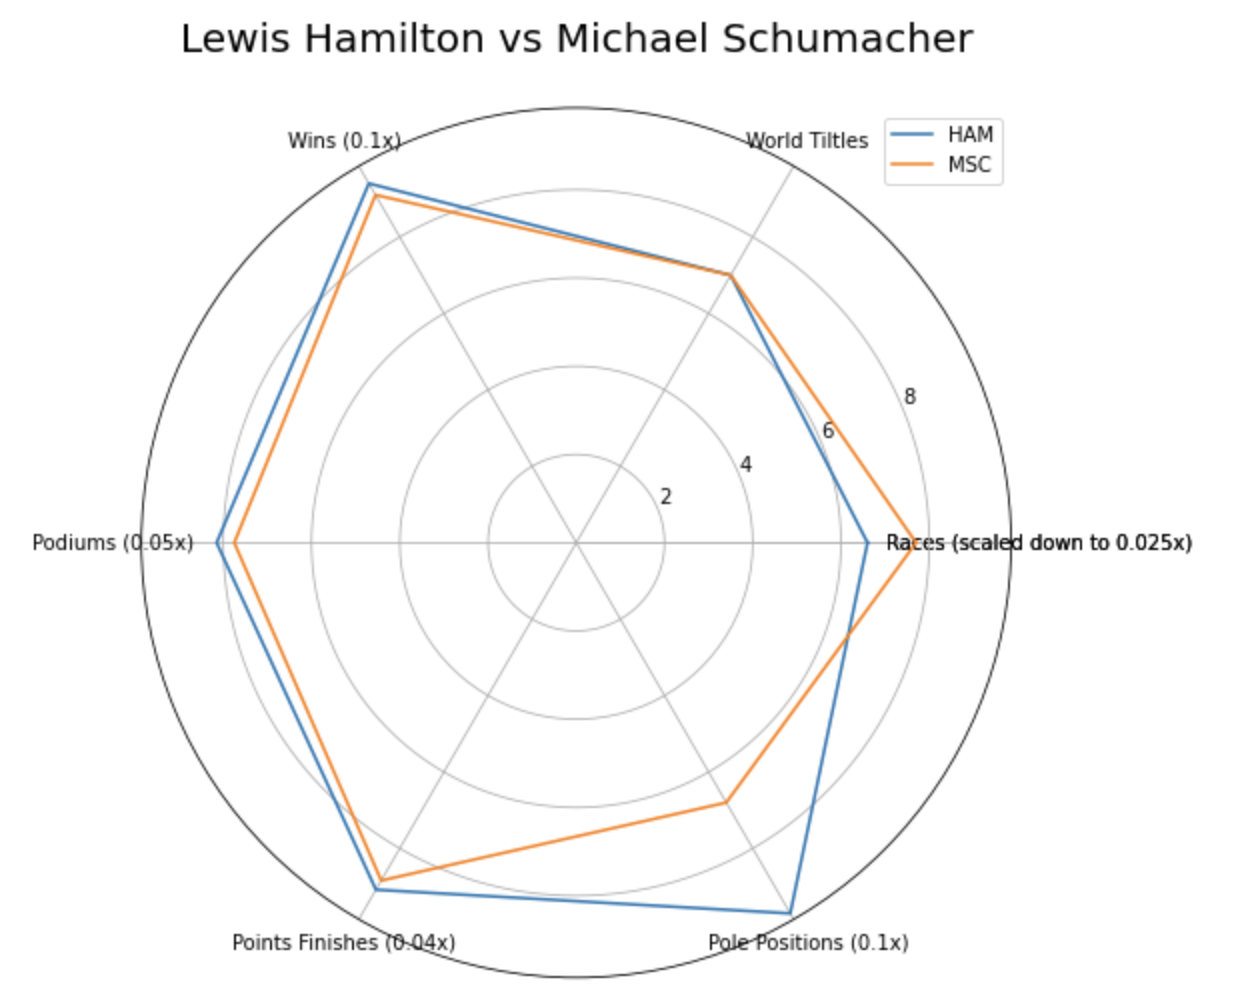
\includegraphics[scale=0.4]{hammsc}
\caption{}
\label{fig:hammsc}
\end{figure}\\\\\\\\\\\
\section{Conclusion:}
\textit{Figure 1:}  From the Bar Graph we can observe the improvement in Hamilton's performance over the years, with better consistency. Over the last couple of years he has consistently been winning the Championship. Bar Graph has been used here to show both the values and comparison. The y-axis has been inverted as a lower magnitude of rank is better.\\\\
\textit{Figure 2:} This pie chart represents Hamilton's performance in the 266 F1 races he has started till date. The numbers are not as important as the percentages in this case, hence the use of pie chart.\\\\
\textit{Figure 3:} From the Heatmap, we can see that Hamilton's performance has been consistently good in Australian, Belgian and Abu Dhabi Grands Prix. In Monaco his performance has been slightly lower, but has improved over time. This is expected as Monaco and Singapore are notoriously tough tracks. Because there are two variables involved, a heat chart is perfect for data like this. It makes it easier to observe trends both across columns and down the rows.\\ Note: Some values have been set as 0. These are the cases of retirement from race(due to car failure/crashes), Disqualification, or disruption in schedule because of the Pandemic.\\\\
\textit{Figure 4:} This scatter plot consists of 242 data points from all the races he completed. We can observe a distinct improvement in his positions since 2013-14, the time when he switched teams. From this scatter plot we can see that the decision has been for the better. A scatter plot is ideal for these cases because the input data is large and we wish to observe trends in data without biases in opinion.\\\\
\textit{Figure 5:} The criteria used here are varied and ideally require different axes, but that would be much cluttered. A radar chart has been used to get a better visual effect. From this chart we can see that Hamilton has better statistical records than Schumacher, though it must be kept in mind that scoring rules, cars, technologies change with time.\\\\
From the stats presented above we can see that Lewis Hamilton is certainly the greatest racing driver of this generation.\\\\\\
\begin{figure}[h]
\centering
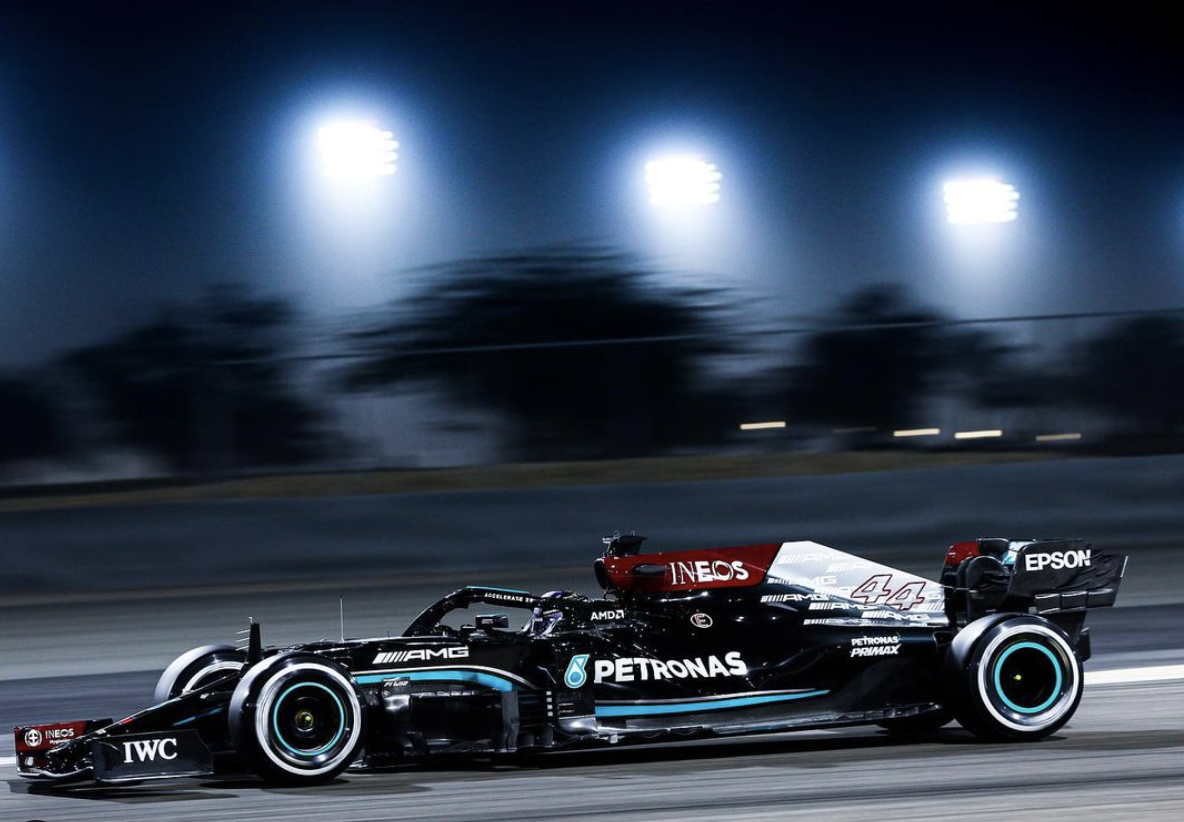
\includegraphics[scale=0.6]{car}
\caption{}
\label{fig:car}
\end{figure}

%\bibliographystyle{plain}
%\bibliography{references}
\end{document}
%125 words left


